\subsubsection{Project}
	In the UPRM system, projects will refer to any new paper or report that the researcher(s) will be involved in. The user has to be able to create multiple projects and keep track of progress by means of a timeline and project specific sub-deadlines.
	The access rights and privileges to each operation will have to be checked before any operation is executed.\\ \\
	\textbf{Use Cases:}
	\begin{itemize}
		\item Creation of Project
		\item Creation of Timeline
		\item Updating of Project
		\item Update of Timeline
		\item Deletion of Project \\
	\end{itemize}
	\textbf{Project Use Case Overview Diagram:}\\
	\centerline{\fbox{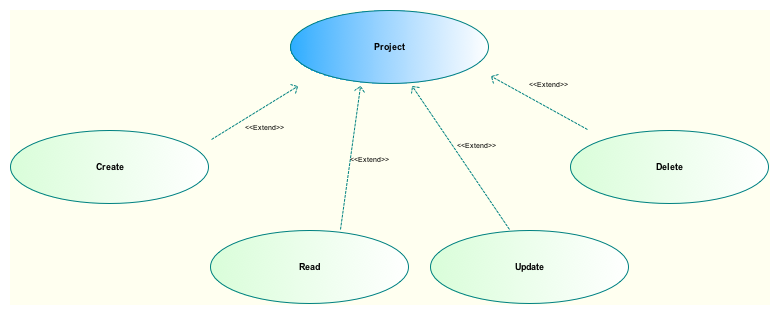
\includegraphics[width=\linewidth]{CRUD/uprm_CRUD_Overview.png}}}		
	